\chapter{Ultrasound}

Mechanical energy in the form of high-frequency (usually in the range
of 2 to 10 MHz)\footnote{The higher the frequency the better
  resolution and image detail, but lower penetration.} sound waves can
be used to generate images of the anatomy of a patient. These waves
pass through tissues, get reflected, and the returning wave (echo) is
detected and forms the image. In B-mode (B for
Brightness\footnote{There is A-Mode (A for Amplitude) that is mainly
  used in mainly in ophthalmology to investigate retinal detachment.})
imaging, the most common imaging used in medicine, the intensity of
the returning wave is represented as a level of brightness on the
monitor to give a 2D cross-sectional image on the monitor
\cite{abdulla2025ultrasound}.

\section{Acquisition details}
The echoes returned are shown on screen in a grey-scale corresponding
to their intensity. The structures are shown as a 2D image on
screen. A short-duration pulse of sound is generated by an ultrasound
transducer that is in direct physical contact with the tissues being
imaged. The sound waves travel into the tissue, and are reflected by
internal structures in the body, creating echoes. The reflected sound
waves then reach the transducer, which records the returning sound
\cite{bushberg2011essential,abdulla2025ultrasound_machine}.

\begin{figure}
  \centering
  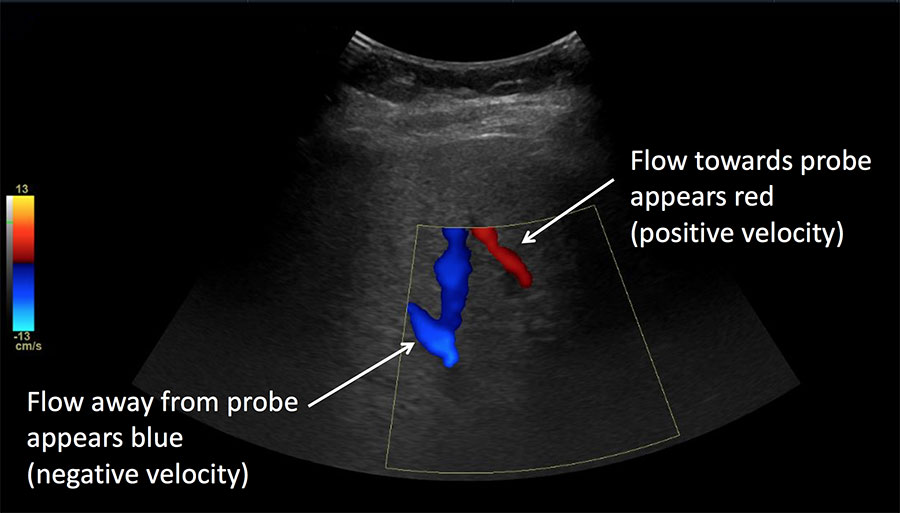
\includegraphics{doppler}
  \caption{An ultrasound image that shows the Doppler effect
    \cite{abdulla2025ultrasound_imaging_doppler}.\label{fig:doppler}}
\end{figure}

The speed of the sound signal in the tissues are low enough to use the
Doppler effect to detect their motion. Thus, for example, using the
M-Mode (M for Motion) we can measure the blood flow displayed as color
channels (see Figure~\ref{fig:}
).\footnote{Both the speed
  and direction of blood flow can be measured, and within a subarea of
  the grayscale image, a color flow display typically shows blood flow
  in one direction as red, and in the other direction as blue
  \cite{bushberg2011essential}.}

\section{Image content}
Ultrasound imaging is basically a 2D technique (slices). However, 3D
images (volumes) can be generated by placing the known voxels in a 3D
structure and interpolating the unknown voxels. Then, using
segmentation it is possible to display surfaces to see, for example,
the face of a fetus.

\section{Speckle noise}
Ultrasound images are noisy and the predominant type of noise is
speckle noise.

Speckle is usually modeled as multiplicative noise. Amplitude
(magnitude) follows a Rayleigh distribution. Phase is uniformly
distributed. Intensity (amplitude squared) follows an exponential
distribution.

If multiple images are taken (changing the angle and orientation) and
averaged, then intensity in the resulting \emph{spatial compounding}
\cite{bushberg2011essential} follows a Gamma distribution.
